\documentclass[11pt, a4paper]{article}
\usepackage[affil-it]{authblk} 
\usepackage{etoolbox}
\usepackage{lmodern}
\usepackage{titlesec}
\usepackage{float}

\makeatletter
\patchcmd{\@maketitle}{\LARGE \@title}{\fontsize{20}{19.2}\selectfont\@title}{}{}
\makeatother

\renewcommand\Authfont{\fontsize{16}{14.4}\selectfont}
\renewcommand\Affilfont{\fontsize{12}{10.8}\itshape}

\title{\textbf{Assignment 1}} 
\author{Pavan R Hebbar - 130010046}
\usepackage{graphicx}
\begin{document}
\maketitle
\newpage
\section{Question1:}
\subsection{2D case}
\subsubsection{Velocity Distribution}
\begin{equation}
 f(\vec{v}) = n\frac{m}{2\pi k T}e^{-\frac{m\vec{v}\cdot\vec{v}}{2kT}}
\end{equation}
\subsubsection{Speed Distribution}
\begin{equation}
 f(v) = n \frac{m}{2\pi k T}ve^{-\frac{mv^2}{2kT}}
\end{equation}

\subsubsection{Energy Distribution}
\begin{equation}
 f(\epsilon) = \frac{n}{2\pi kT}e^{-\frac{\epsilon}{kT}}
\end{equation}

Mean velocity:
\begin{equation}
 V_{mean} = \sqrt{\frac{kT}{8\pi m}}
\end{equation}

Rms velocity:
\begin{equation}
 V_{rms} = \frac{kT}{\pi m}
\end{equation}


\subsection{1D case}
\subsubsection{Speed Distribution:}
\begin{equation}
 f(v) = n\sqrt{\frac{m}{2\pi kT}}e^{-\frac{mv^2}{2kT}}
\end{equation}
\subsubsection{Energy Distribution}
\begin{equation}
 f(\epsilon) = n\frac{1}{2\sqrt{\pi k T}}\frac{1}{\sqrt{\epsilon}}e^{-\frac{\epsilon}{kT}}
\end{equation}

Mean velocity:
\begin{equation}
 V_{mean} = \sqrt{\frac{2kT}{\pi m}}
\end{equation}

RMS velocity:
\begin{equation}
 V_{rms} = \frac{kT}{4m}
\end{equation}

\section{Question 2:}
(Refer code)
\section{Question 3:}
\begin{figure}[H]
 \centering
 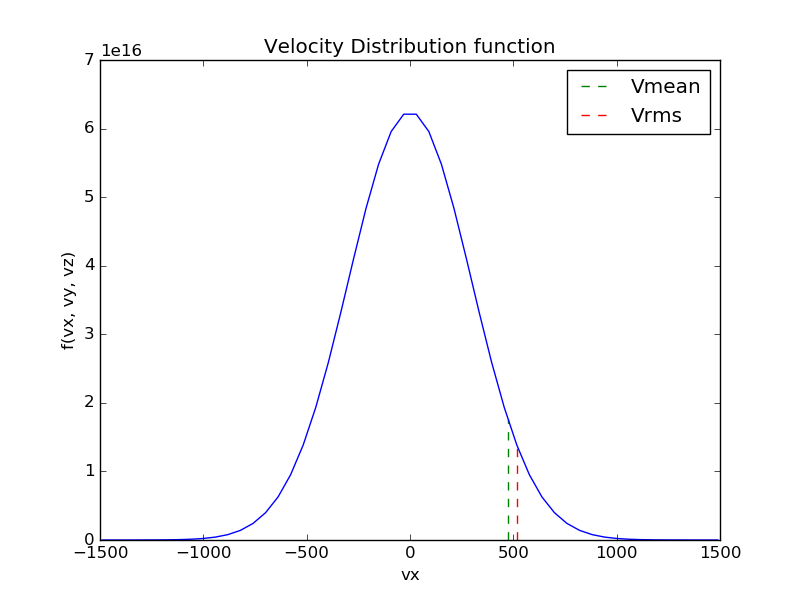
\includegraphics[scale = 0.5]{f_vel.png}
 \caption{Velocity Distribution Function}
 \label{fig:vel_pdf}
\end{figure}

\begin{figure}[H]
 \centering
 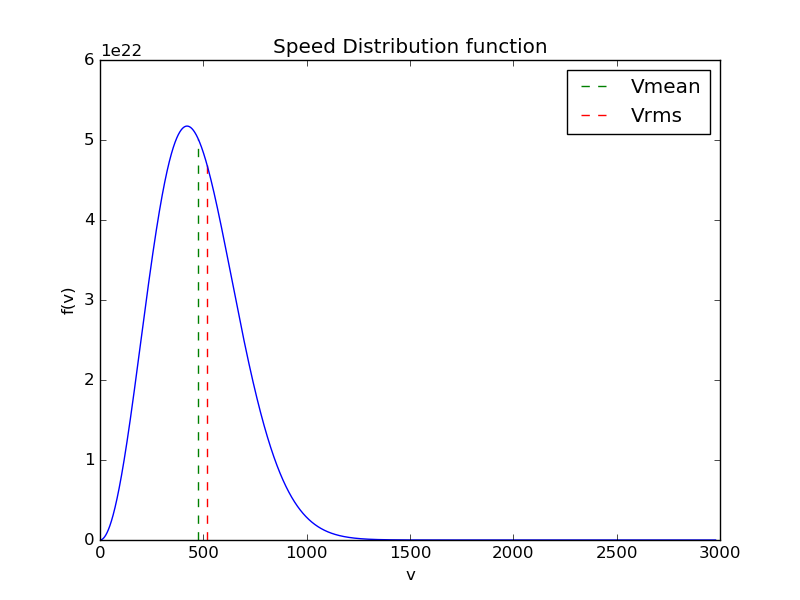
\includegraphics[scale = 0.5]{f_speed.png}
 \caption{Speed Distribution Function}
 \label{fig:speed_pdf}
\end{figure}

\begin{figure}[H]
 \centering
 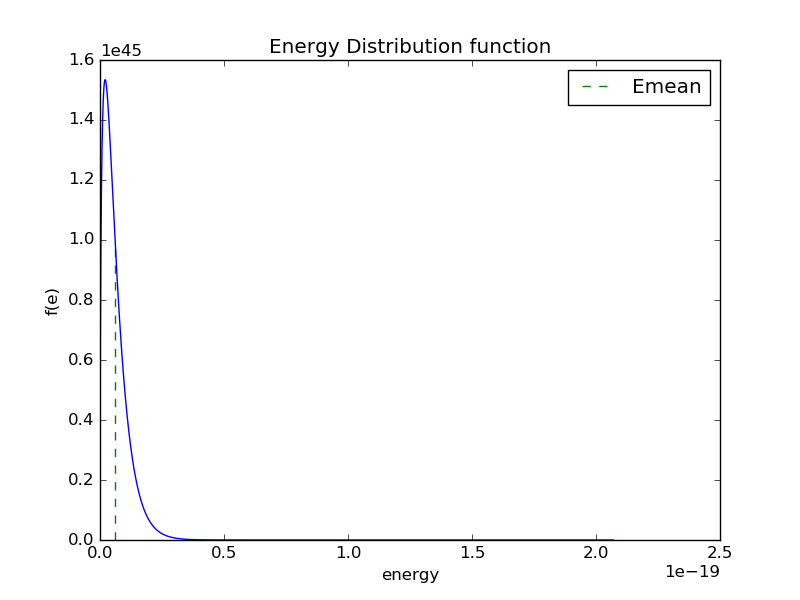
\includegraphics[scale = 0.5]{f_energy.png}
 \caption{Energy Distribution Function}
 \label{fig:energy_pdf}
\end{figure}

\section{Question 4:}
(Done in the above plots)
\section{Question 5:}
(Refer code) \\
The values  given below are for 20000 grids in velocity and energy \\
Pressure = $1.087 \times 10^5 Pa$ \\
Energy = $8.150 \times 10^4 J$ \\
Vmean = $475.321 m/s$ \\
Entropy = $1.36 \times 10^27$\\


\section{Question 6:}
(Refer code)
We see that the mean velocity and the pressure are almost independent of grid size. The error in Pressure and the Mean 
velocity was of the order of $10^-9$ and $10^-11$ respectively. So the pattern of the graph isn't of much relevence
as the values of Boltzmann constant and the Avagadro number are taken only till 2 decimal places

\begin{figure}[H]
 \centering
 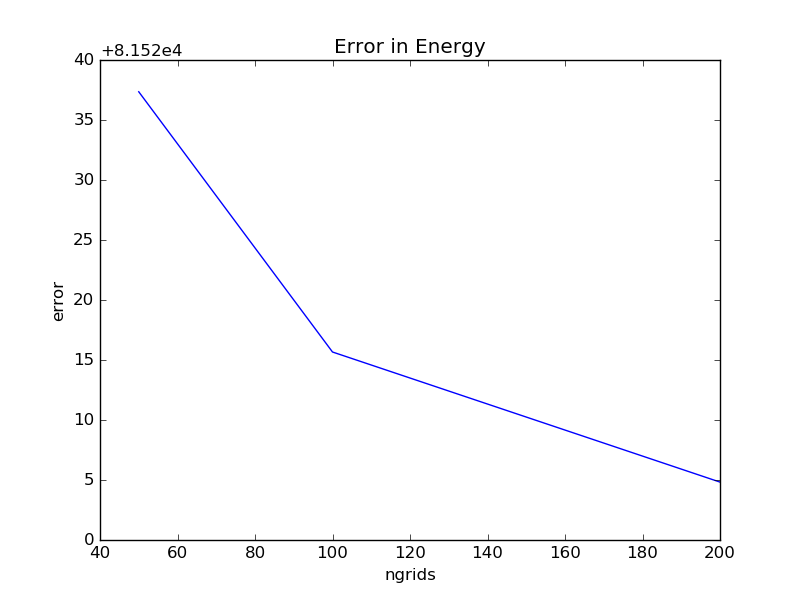
\includegraphics[scale = 0.5]{Error_e.png}
 \caption{Error in energy calculation}
 \label{fig:energy_error}
\end{figure}

\begin{figure}[H]
 \centering
 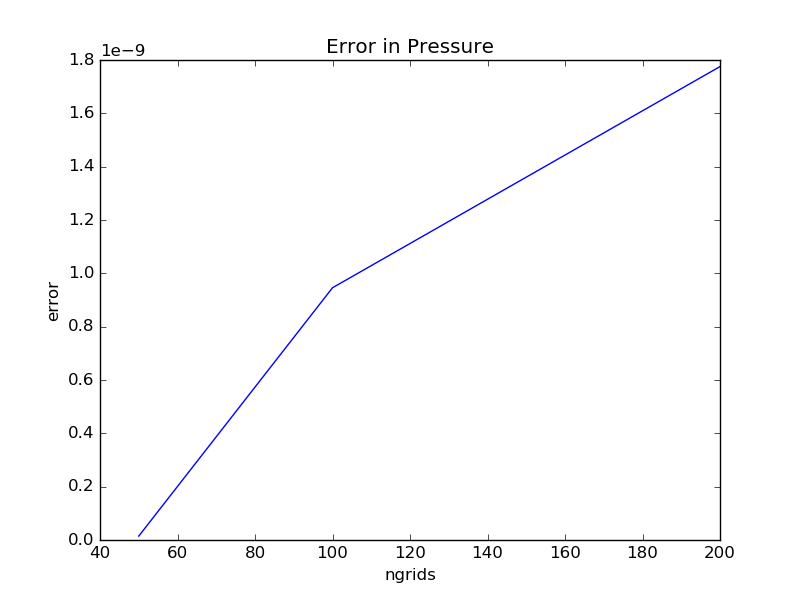
\includegraphics[scale = 0.5]{Error_p.png}
 \caption{Error in pressure calculation}
 \label{fig:pressure error}
\end{figure}

\begin{figure}[H]
 \centering
 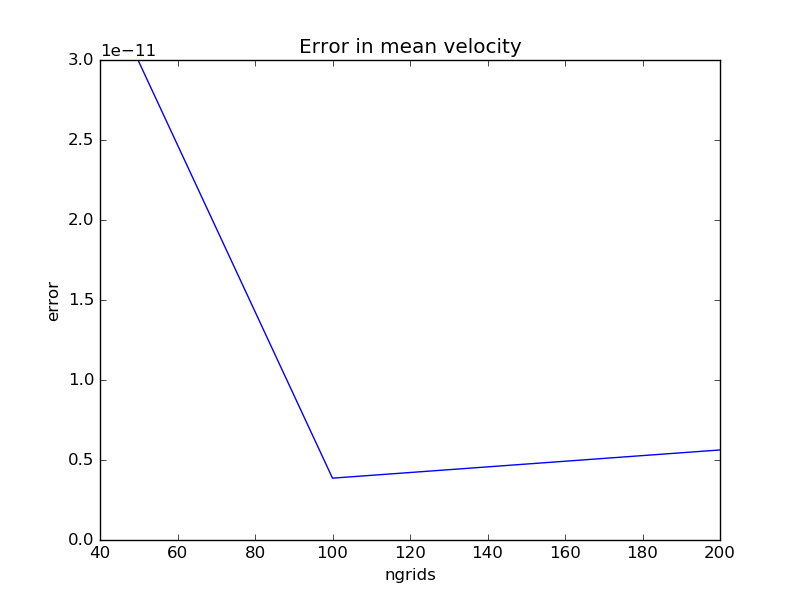
\includegraphics[scale = 0.5]{Error_v.png}
 \caption{Error in mean velocity}
 \label{fig:vmean error}
\end{figure}

\section{Question 7:}
Following functions were chosen
\begin{itemize}
 \item Exponential fucntion \\
  Entropy = $-4.57 \times 10^30$
 \begin{equation}
  p(x) = e^{-x}
 \end{equation}
 \item Exponential Logarithmic function: $p  = 0.5$; $\beta = 2$\\
  Entropy = $-1.33 \times 10^31$
 \begin{equation}
  p(x, p, \beta) = \frac{-1}{ln(p)} \frac{\beta (1-p)e^{-\beta x}}{1 - (1-p)e^{-\beta x}}
 \end{equation}
 \item Levy Distribution: $\mu = 0$, $c = 2$ \\
 Entropy = $4.52 \times 10^27$
 \begin{equation}
  p(x;\mu, c) = \sqrt{\frac{c}{2*np.pi}}\frac{e^{\frac{c}{x - \mu}}}{(x - \mu)^{3/2}}
 \end{equation}
\end{itemize}
(Results are weird, not able to justify/find the bug)

\section{Question 8:}
V has been plotted in logarithmic scale. Blue is for ions and red for electrons
\begin{figure}[H]
 \centering
 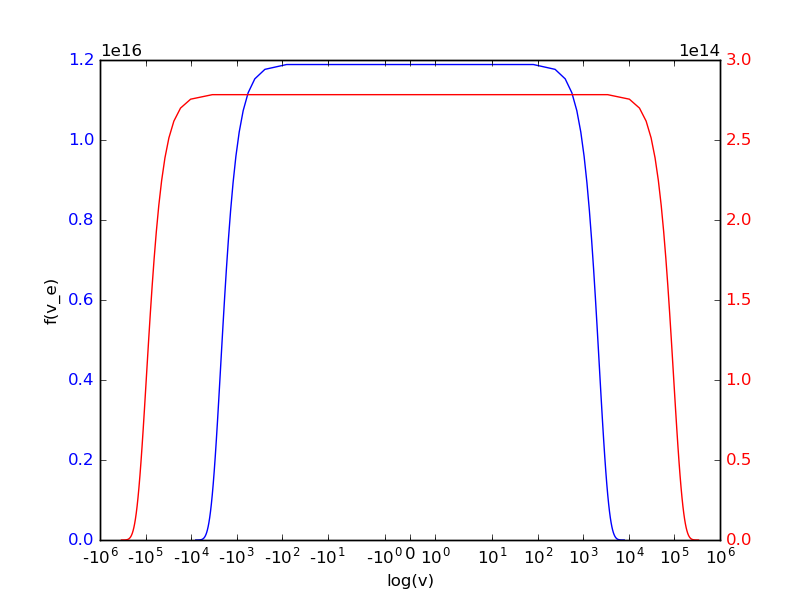
\includegraphics[scale = 0.5]{Plasma_vel.png}
 \caption{Velocity PDF of electrons and ions}
 \label{fig:plasma_v}
\end{figure}

\begin{figure}[H]
 \centering
 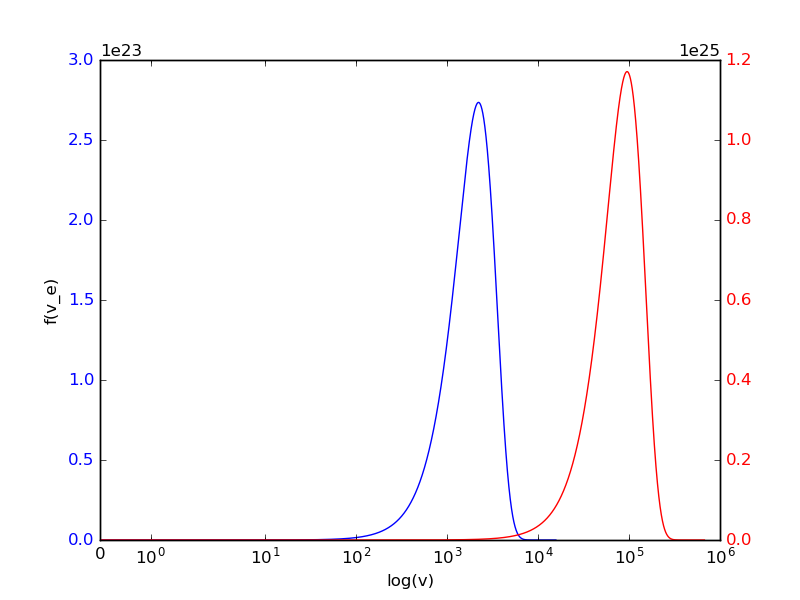
\includegraphics[scale = 0.5]{Plasma_speed.png}
 \caption{Speed pdf of electrons and ions}
 \label{fig:plasma_s}
\end{figure}


\begin{figure}[H]
 \centering
 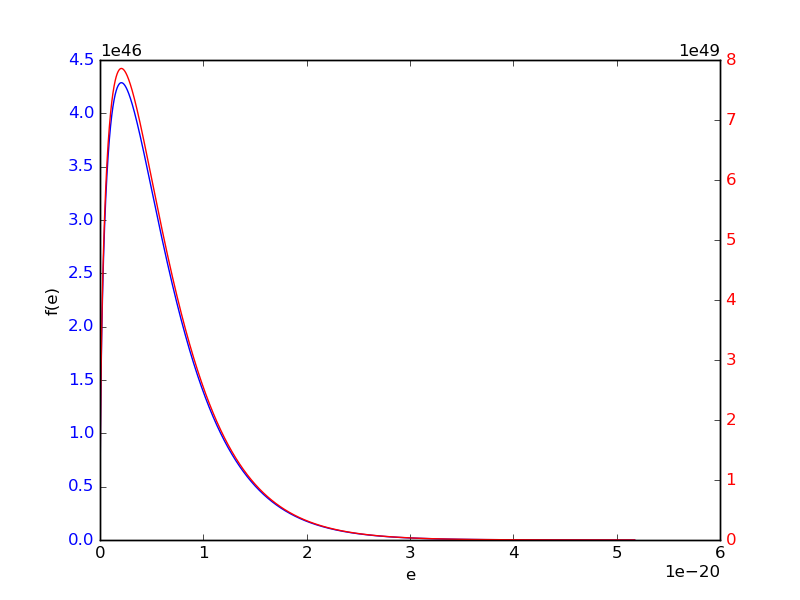
\includegraphics[scale = 0.5]{Plasma_energy.png}
 \caption{Energy PDF of electrons and ions}
 \label{fig:plasma_e}
\end{figure}





\end{document}